\documentclass[10.5pt, twocolumn]{article}

\usepackage[english]{babel}
\usepackage{graphicx}
\usepackage{imakeidx}
\usepackage{mathrsfs, amsmath}
\usepackage{systeme}
\usepackage{array}
\usepackage[utf8]{inputenc}
\usepackage{siunitx}
\usepackage{booktabs}
\usepackage{adjustbox}
\usepackage{geometry}
\geometry{a4paper,total={145mm,210mm}}
\usepackage{makecell}
\usepackage{afterpage}
\usepackage{listings}
\usepackage{subcaption}
\usepackage[toc,page]{appendix}
\usepackage[table]{xcolor}
\usepackage{pifont} % ding symbols
\usepackage{tikz}
\usepackage{changepage}
\usepackage{multirow} % multi row in tables
\usepackage{booktabs}
\usepackage{textcomp} % registered and copyright symbol
\usepackage{lscape} % vertical instead to horizontal
\usepackage{longtable} % for more page tables
\usepackage{eurosym}
\usepackage{lmodern}
\usepackage{amstext}
\usepackage{pdfpages} % import pdf pages
%\usepackage[hidelinks]{hyperref} % delete ugly hyperref borders of hyperlink
\usepackage{hyperref} % internal hyperlinks
\usepackage{titling} % titles
\usepackage{titlesec} % subtitles
\usepackage{blindtext} % for casual texts
\usepackage{dblfloatfix} % forces image at bottom in two-column files
\usepackage{gensymb} % standard unit of measurement
\usepackage{enumitem}

\DeclareRobustCommand{\officialeuro}{%
  \ifmmode\expandafter\text\fi
  {\fontencoding{U}\fontfamily{eurosym}\selectfont e}}



\makeindex[columns=2, title=Indice alfabetico, options= -s mystyle.ist, intoc]

\newcommand*{\Scale}[2][4]{\scalebox{#1}{\ensuremath{#2}}}
\renewcommand*\contentsname{Indice}
\newcommand*\NewPage{\newpage\null\thispagestyle{empty}\newpage}
\newcommand{\Virgolette}[1]{``#1''}
\newcommand*\circled[1]{\tikz[baseline=(char.base)]{
	\node[shape=circle,draw,inner sep=2pt] (char) {#1};}}
\newcommand{\tikzcircle}[2][red,fill=red]{\tikz[baseline=-0.5ex]\draw[#1,radius=#2] (0,0) circle ;}%command for draw text circle coloured
\def\changemargin#1#2{\list{}{\rightmargin#2\leftmargin#1}\item[]}
\let\endchangemargin=\endlist
\makeatletter
\let\originalpart=\part



\newcolumntype{C}[1]{>{\centering\arraybackslash}p{#1}}
\newcolumntype{L}[1]{>{\arraybackslash}p{#1}}
\newcolumntype{R}[1]{>{\raggedleft}p{#1}}
\newcolumntype{G}[1]{>{\centering\arraybackslash\columncolor{gray0}}p{#1}}

\definecolor{gray0}{gray}{0.9}
\definecolor{gray1}{gray}{0.7}
\definecolor{gray2}{gray}{0.4}

\lstset{
	literate = {α}{{$\alpha$}}1 {∆}{{$\Delta$}}1 {θ}{{$\theta$}}1 {η}{{$\eta$}}1 {→}{{$\rightarrow$}}1 {∂}{{$\partial$}}1, %tutti i simboli da usare come codice
	language = Mathematica % linguaggio
}
\hypersetup{
	citebordercolor=red
}


% ----- TITLE
\titleformat*{\section}{\Large\bfseries}
\title{
	\large{University of Trento}\\
	\normalsize{Master in Mechatronics Engineering}\\
	\vspace{0.2cm}
	\large{\textit{Modelling and Simulation of Mechatronics Systems}}\\
	\vspace{0.2cm}
	\Large{\textbf{Development, analysis and optimization of the performance of an innovative driving simulator}}\\
	\vspace{0.25cm}
	\hrule
	\vspace{0.2cm}
	\large{\textbf{Kinematic analysis}}\\	% Title
	\vspace{0.2cm}
	\hrule
}
\author{A. Comoretto \and J. Losi \and S. Valentini}
\date{\vspace{0.5cm}}
% ----- TITLE


\begin{document}
\maketitle

The kinematic analysis...

\section{Kinematic equations}
In this section the mechanism's behaviour is studied.
In Figure \ref{f:Top-View} is shown the top view of the mechanism.
\begin{figure}[h!]
	\centering
	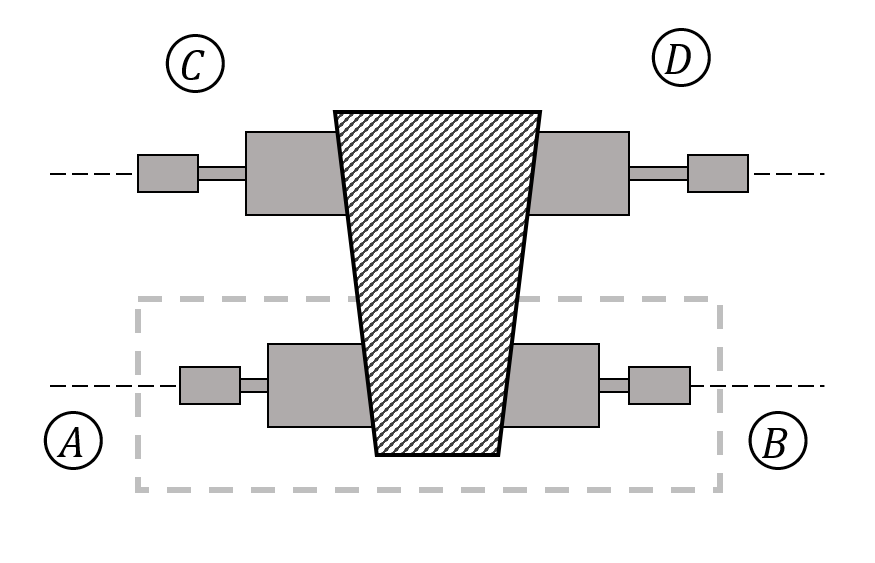
\includegraphics[width=7cm]{Images/Mechanism_TopView}
	\caption{Top view of the full-mechanism.}
	\label{f:Top-View}
\end{figure}

In first approximation a 2D analysis is conduced, and is refered only to the bodies \circled{A} and \circled{B}.

\subsection{2D-kinematic analysis}
The mechanism studied in the 2D simplification is the merked part in Figure \ref{f:Top-View}, in fact only bodies \circled{A} and \circled{B} are taken into account, and the result is shown in Figure \ref{f:2D_Mechanism}.
\begin{figure}[h!]
	\centering
	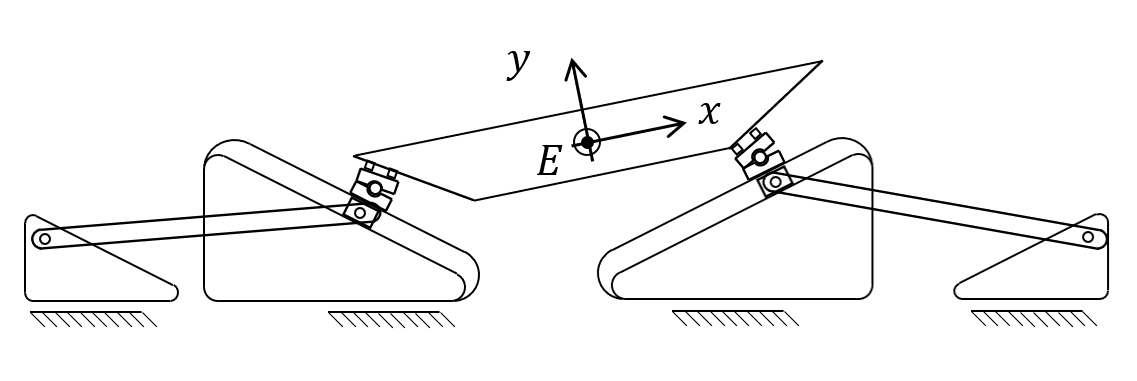
\includegraphics[width=7cm]{Images/Mechanism_LateralView}
	\caption{2D mechanism.}
	\label{f:2D_Mechanism}
\end{figure}

For the 2D analysis it is choosen to consider the length of the platform as a constant, even if it could be variable, due to its geometry.
More complex analysis are made in the following Section \ref{s:3D-kinematic} during the 3D analysis.

Thanks to this consideration it is possible to say that the full-mechanism is composed by two mirrored sub-mechanisms, made by four sub-bodies, joined by the platform.
So the sub-mechanism studied is shown in Figure \ref{f:Sub-Mechanism}.
\begin{figure*}[h!]
	\centering
	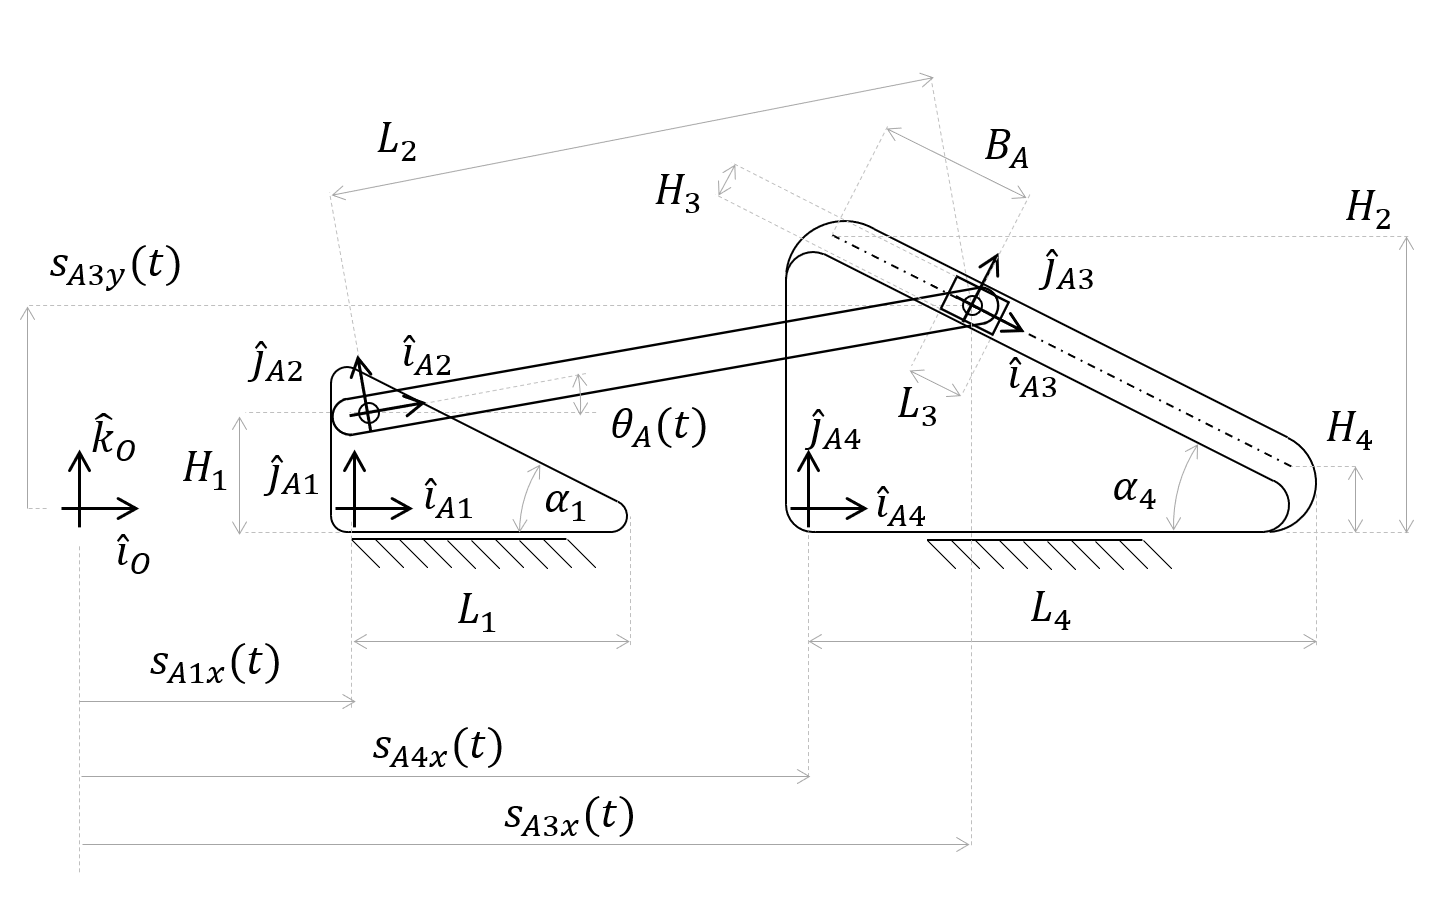
\includegraphics[width=12cm]{Images/Sub-Mechanism}
	\caption{One of the four sub-mechanism of the structure.}
	\label{f:Sub-Mechanism}
\end{figure*}
The same can be done for all the other sub-mechanisms by changing the subscripts.

At a first sight, it is easy to say that the four motors will be the independant variables, they are:
\begin{itemize}
  \item \( s_{A1x}(t) \);
  \item \( s_{A4x}(t) \);
  \item \( s_{B1x}(t) \);
  \item \( s_{B4x}(t) \).
\end{itemize}
Although the simplicity of this consideration it has to be revisited in way to work together with the previous one: in fact consider the length of the platform (named \( L_5\)) constant, means that one of the motor has to become a dependant variable.

In particular \( s_{B1x}(t) \) is considered the dependant variable.
\subsection{3D-kinematic analysis}
\label{s:3D-kinematic}

\section{Velocity analysis}
Regarding the velocity analysis it was decided to operate in the following way.
At first, after have obtained from the position analysis the following three objects:
  \begin{itemize}
    \item \( Phi_{tot}\): complete set of constraint equations;
    \item \( qI_{tot}\): set of independent variables;
    \item \( qD_{tot}\): set of dependent variables;
  \end{itemize}
three dependent variables (\(EE_{x}(t)\), \((EE_{y}(t)\),\((EE_{angle}(t)\)) were added to the set of dependent variables and clearly to set of constraint equations. The aim was to obtain directly the velocity ratios related to these variables, that are the X position, the Y position and the roll angle of the center of mass of the platform that was tought as the position of an eventual driving position.
If that had not been done , we would obtain velocity ratios related  to other internal variables, such as the angles of the bars and the positions of the rolleys.
At this point, in order to perform the Jacobians, we dropped the time dependency and after that, a function to restore the dependency w.r.t. the time was created, required to compute the derivation later.
Furthermore the Jacobians w.r.t. the dependent and independent coordinates has been computed and thus the matrix of velocity ratios (\(tau\)) was calculated exploiting the Jacobians.
Secondly it was developed the section for the plot of velocity ratios as a function of the independent variables, that are the position of the three actuators (because as already said, supposing a constant value of the length of the platform, one can be considered as \Virgolette{dummy}). In that section, not all the velocity ratios were plotted but only the ones related to the X and Y position of the end effector and to its roll angle because those one were the only one really significative for our analysis.
Speaking about that section, a procedure for the plots called \textit{velocity\textunderscore plot} was made. More specifically the procedure takes as inputs:
  \begin{itemize}
    \item \( EE\textunderscore number \): chosen number between 1 and 3 that identifies the correct end effector variable (X, Y or angle);
    \item \( actuator\textunderscore number\): desired actuator variable w.r.t whom we choose to plot the solution;
    \item \(actuator\textunderscore extremes\): two elements vector that identifies the extreme postions of the desired actuator;
    \item \(constant\textunderscore actuators\textunderscore values \): two values vector that identifies the values to be assigned by the two actuators that remain constant.
  \end{itemize}
and gives as outputs the trasmission ratios between X, Y position and angle of the end effector and the actuators as a function of one of the three independent DoF, assuming the other two as constants.
As third main point it was decided to plot, besides the velocity ratios, also the pure velocities of the X, Y position of the end effector and its roll angle w.r.t. the position of one of the three DoF. In that case, as the requests specified, the velocity of the active actuator was fixed to one while the position of the other two actuators was mantained in the initial position.
In order to develop this part, at first, it was calculated analitically the velocity of the dependent coordinates solving the derivative w.r.t. time of the equation of the complete set of constraints considering as unkonwns the derivative w.r.t. time of the complete set of dependent coordinates. Then, in the solution obtained, was substituted the chosen solution of the kinemtics found before.

\section{Acceleration analysis}
Regarding the acceleration analysis, this part was quite similar to the one made before. As a matter of fact, having the analitical solution of the kinematics, in order to obtain the expression of the acceleration of the dependent coordinates it was solved the double derivative w.r.t. time of the complete set of constraints considering as unkonwns the double derivative w.r.t. time of the complete set of dependent coordinates.
After that, the chosen solution of the kinematics was substituted into the expression of the dependent acceleration in order to obtain them as dependent only to the independent variables.
Moreover the acceleration of the X, Y coordinates and of the roll angle of the end effector was plotted w.r.t the position of each one of the three DoF (mantaining the other two fixed at each time). Furthermore, as the the requests specified, the velocity and the acceleration of the moving actuator, that was considered for each plot, were fixed to an unitaty value. 
\section{Effects of the main geometrical parameters}


\begin{thebibliography}{}
\bibitem{aVDS}
\Virgolette{\textit{Advanced Vehicle Driving Simulator}}, \textsc{ABDynamics}.

\bibitem{CKAS}
\Virgolette{\textit{6DOF Motion System}}, \textsc{CKAS}.

\bibitem{Kasim}
M. Kasim A. J., \Virgolette{\textit{Design and development of 6-dof motion platform for vehicle driving simulator}}, Universiti Teknologi Malaysia.
\end{thebibliography}
\end{document}
